\chapter[]{Practical exercises}

\label{section:PE}
This section contains and discusses some questions showed in the "Practical Exercises" (PE) lectures, whose answers are not uploaded by the professor. These questions come from past exams and are generally representative of what will appear in the exam.

\section{Practical exercise 1: 15 oct 2025}
These lectures do not bring new topics: they test us on topics already discussed in the lectures. They are propaedeutical for the exam, because they contain both multiple choice and open questions.

Important takeaways form this lecture:\\
\textbf{Basic security part:}
\begin{itemize}
    \item Identification $\neq$ authentication
    \item The hash (digest) must be stored in a \textbf{secure storage}.
\end{itemize}

\textbf{Attacks:}
\begin{itemize}
    \item A replay attack can re-send data even if it has been encrypted.
    \item Denial of Service can also happen when a node is not connected to the internet, for example if the attacker injected a malware on the victim so the victim is blocked. In fact, DoS is still a widely encountered attack.
    \item A virus replicates itself by attaching to another program; a worm does so autonomously, without other programs.
\end{itemize}


\section{Practical exercises 2: 29 oct 2025}
In stream algorithms, the key is not always the same, it always gets changed.

In the exam, it's not enough to indicate like "AES" if we want to use a specific algorithm. Instead, we should indicate the key length and the block mode, like AES-256-ECB

When the exam asks "which mode are we using in these figures", first look at IV to see if it's present. CFB and OFB are not used anymore.

In CBC, if I don't have C1 I can't decrypt C1 of course, because it depends on C1. But if I don't have C1 it doesn't mean that I can't decrypt all the others, because to decrypt a current block I only need the block preceding it.

\paragraph{question (0.5 points at exam)}
If you encrypt 50 bytes of data with AES-128-CBC, how big is the result?

Answer: to encrypt we have to divide data in blocks. Remember AES always uses 128 bit blocks (not depending on the key length), so that's what we do. Then, we encrypt the blocks.

Basically we see that to split 50 bytes with 128-bit blocks, we need to add 14 bytes of padding to the last block, so the answer is 64.

\paragraph{Variant}
If the data to be encrypted is exactly a multiple of the size of the block, \textbf{we still add a full block of padding} in that case. This is done to avoid confusion about where the data ends and where the padding begins.

Of course, with CTR we don't do padding because we can encrypt data bit by bit.

\paragraph{exam question}
Besides the cleartext, we need to also send \textbf{the initialization vector}if we're using CBC. How big is it? It has the size of the \textbf{blocks} of the algorithm, so if we use AES it's 128 bits (16 bytes).

\paragraph{Other things to remember}
\begin{itemize}
    \item never use ECB to encrypt large amounts of data, such as 1 tb.
    \item CBC mode increases the size on disk: the ciphertext size will be greater than the cleartext size.
    \item 3DES can be safe if using 168 bit-key, but it's very slow to encrypt.
    \item if we can, \textbf{always use stream algorithms}, not block ones.
\end{itemize}

\paragraph{Exam question}

\begin{figure}[!ht]
    \centering
    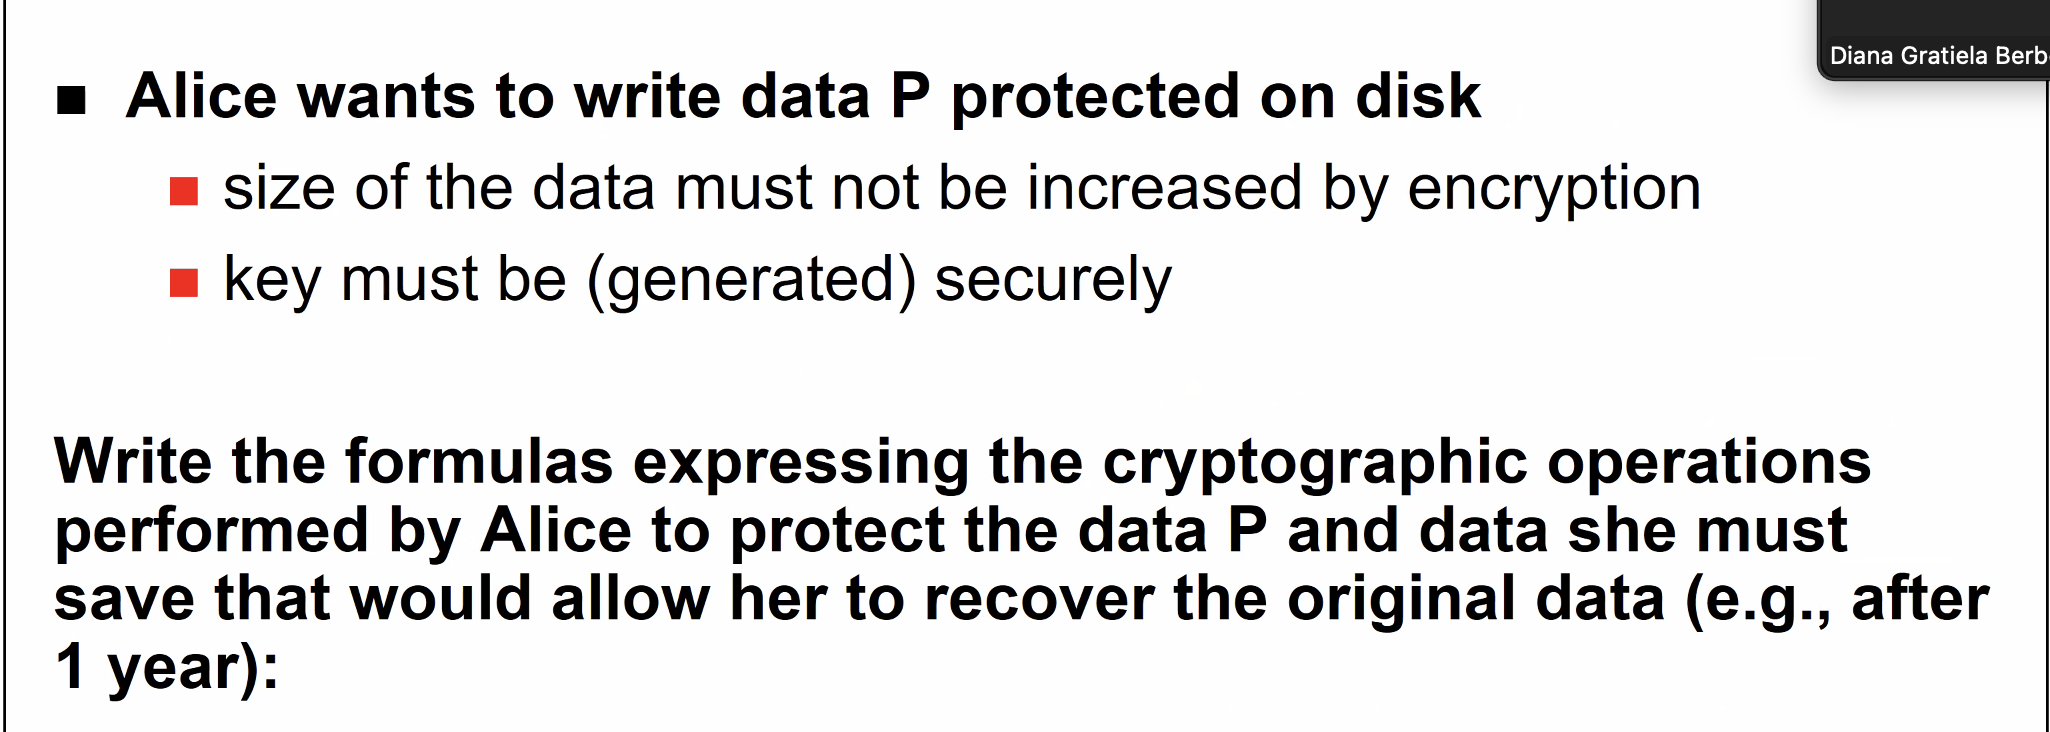
\includegraphics[width=0.5\linewidth]{res/png/scary.png}
    \caption{}
    \label{}
\end{figure}

Answer:
\begin{itemize}
    \item size not increased $\to$ use counter mode (CTR) or cipher text stealing (CTS)
    \item Alice must generate her key. To do this, she can choose a password and a random salt, and the key is generated from these, with the PBKDF2 pseudo-random function.
\end{itemize}

\begin{figure}[!ht]
    \centering
    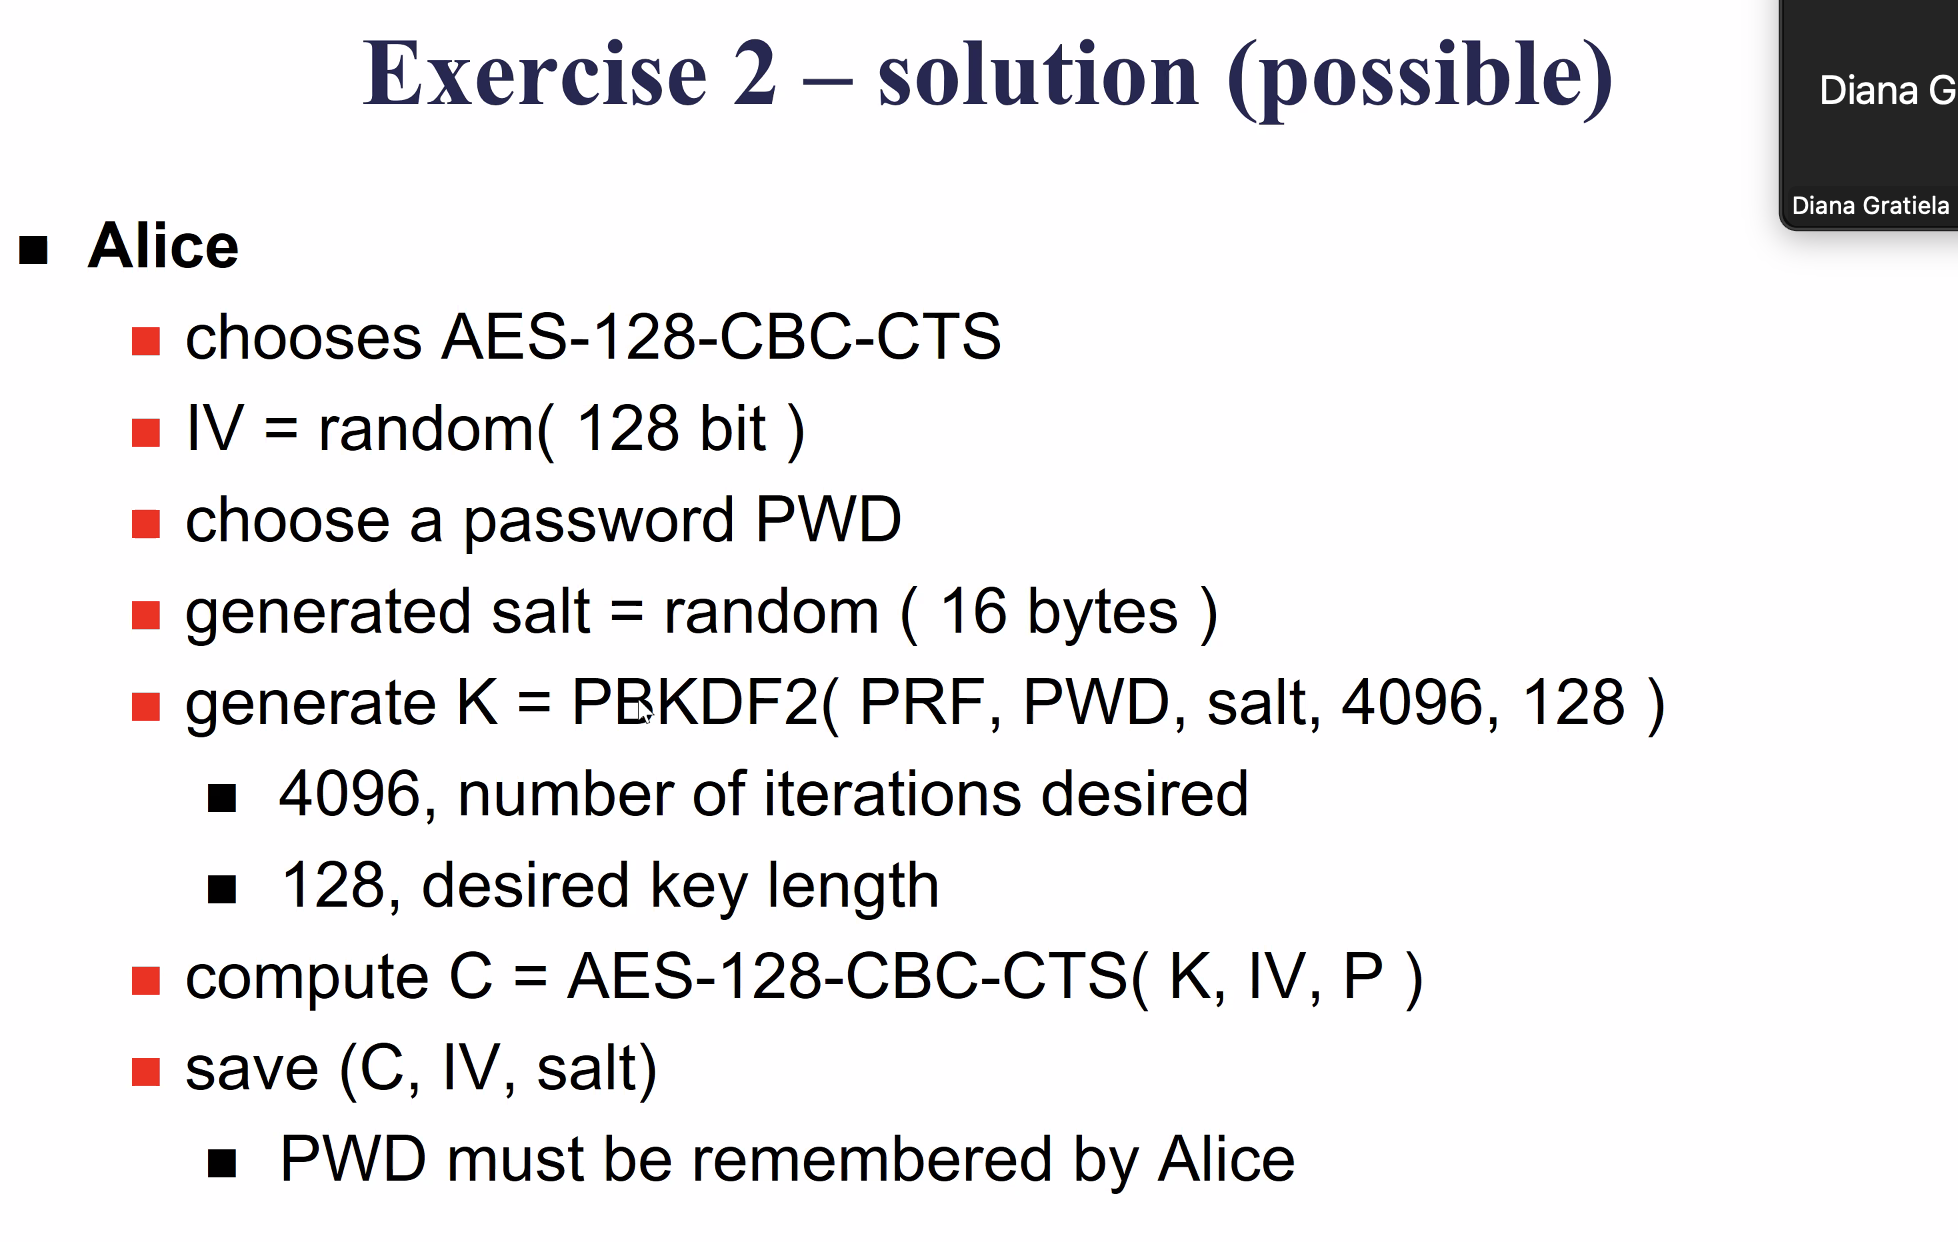
\includegraphics[width=0.5\linewidth]{res/png/fullcount.png}
    \caption{}
    \label{}
\end{figure}

Important: when she wants to recover data after 1 year, she will need the IV and the salt, in order to both decrypt ant get back the key from the same password.

In this kind of exercises it's important to select the right algorithm, write in the correct way, and write the right parameters in the right order.

\subsubsection{Asymmetric crypto}

\begin{itemize}
    \item We can use RSA to do digital signature \textbf{and} key exchange, and of course for encryption. \textbf{it does not provide key agreement}, but key \textbf{encryption}! For key agreement we need DH, which is asymmetric.
    \item we can't USE DSA to encrypt, only to create digital signatures.
\end{itemize}

Other important question on SHA-2:

\begin{figure}[!ht]
    \centering
    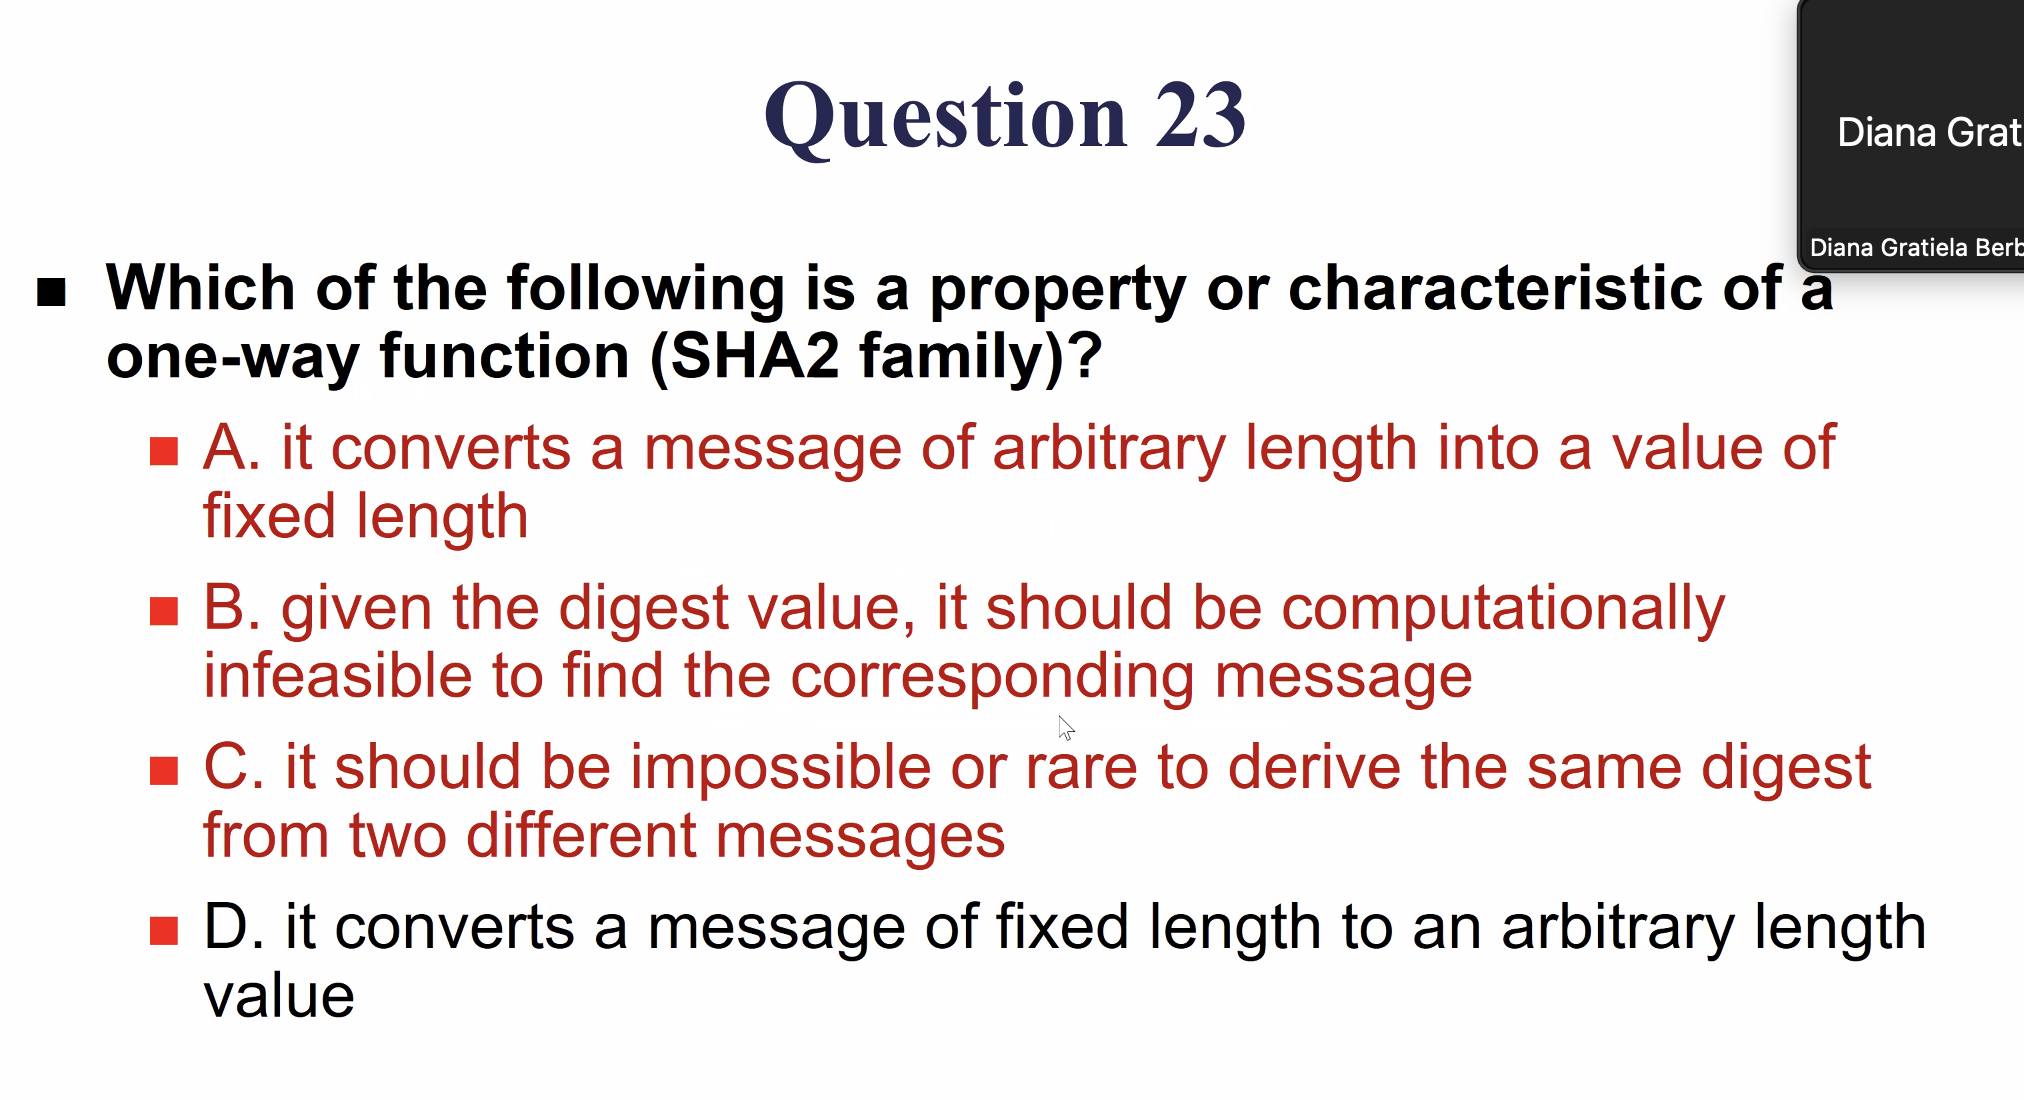
\includegraphics[width=0.8\linewidth]{res/png/shash.png}
    \caption{}
    \label{}
\end{figure}

Where B is invertibility and C is the collision.


\section{PE 3: 12/11/2025}

Birthday paradox:

\begin{figure}[!ht]
    \centering
    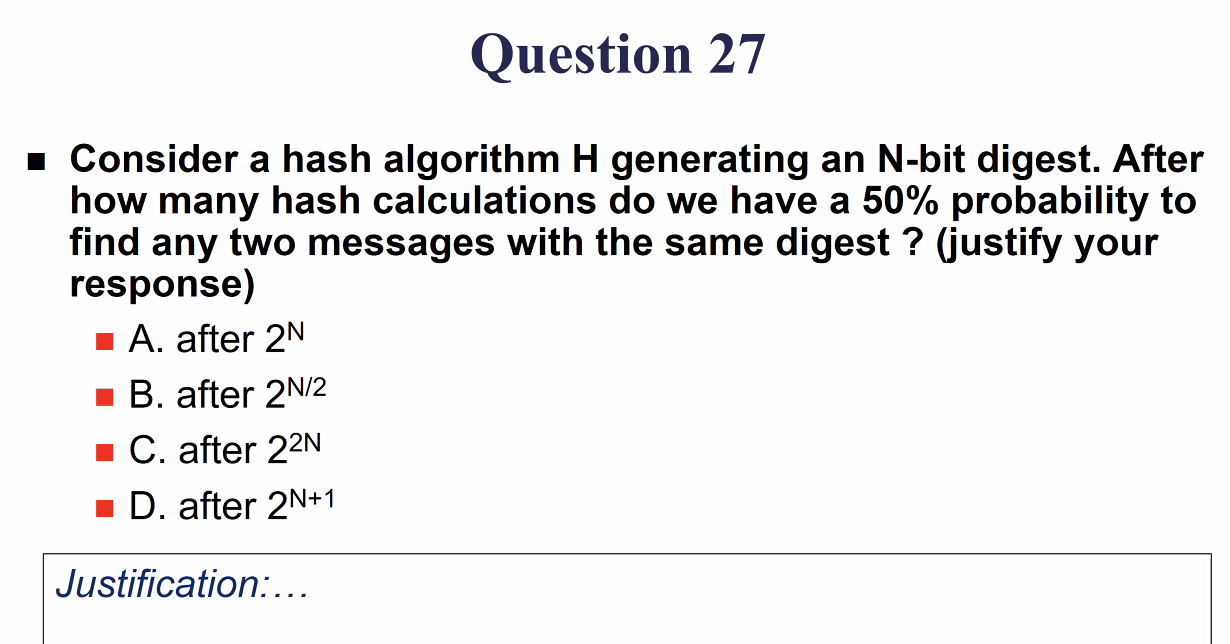
\includegraphics[width=0.5\linewidth]{res/png/bp.png}
    \caption{}
    \label{}
\end{figure}

Other things:
\begin{itemize}
    \item Keyed-digest algorithms, such as those used to create a Hash-based Message Authentication Code (HMAC), use \textbf{symmetric} keys (not asymmetric ones!!). This is because they use a single, shared secret key for both "signing" (generating the digest) and verifying the digest.

    \item The difference between HMAC and CBC-MAC: they both provide integrity and data authentication, but HMAC uses a hash function, while CBC-MAC uses a block encryption algorithm. In fact, CBC-MAC still produces a piece of data that's used like a digest, but it's just an encrypted block.

    \item we must know advantages and disadvantages of EtA, AtE, and A\&E

    \item Authenticated encryption (AEAD) does just \textbf{one} step with just \textbf{one} key.
\end{itemize}


This problem was at the September 2025 exam:

\begin{figure}[!ht]
    \centering
    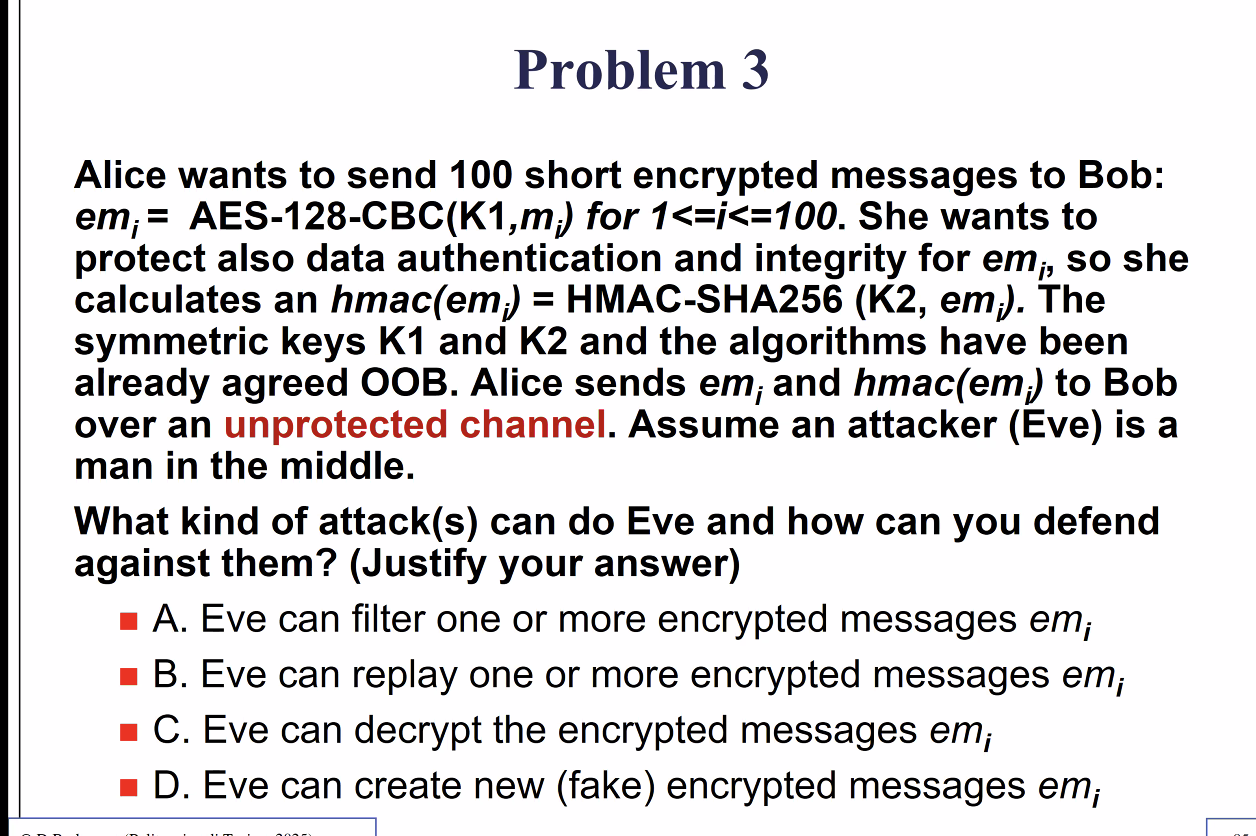
\includegraphics[width=0.5\linewidth]{res/png/epr.png}
    \caption{}
    \label{}
\end{figure}

Answer:
\begin{itemize}
    \item Eve cannot decrypt because she doesn't know $K_1$ and the encryption algorithm used.

    \item She can't create fake messages, because, once again, she doesn't know the keys (she needs $K_2$ to generate a convincing HMAC)

    \item Can she replay? Yeah, because from the exam text alone there's no counter (there's no sequence number). That's why in TLS they put a counter to counter replay attacks.

    \item She can also filter.
\end{itemize}
A solution is a non-repeating nonce or timestamp (anything that resembles a counter), so the receiver can detect if a message is missing (to counter filtering) or repeated (to counter replay).

\paragraph{Ex 3}
.. non l'ho letto ..

here's the solution:

\begin{figure}[!ht]
    \centering
    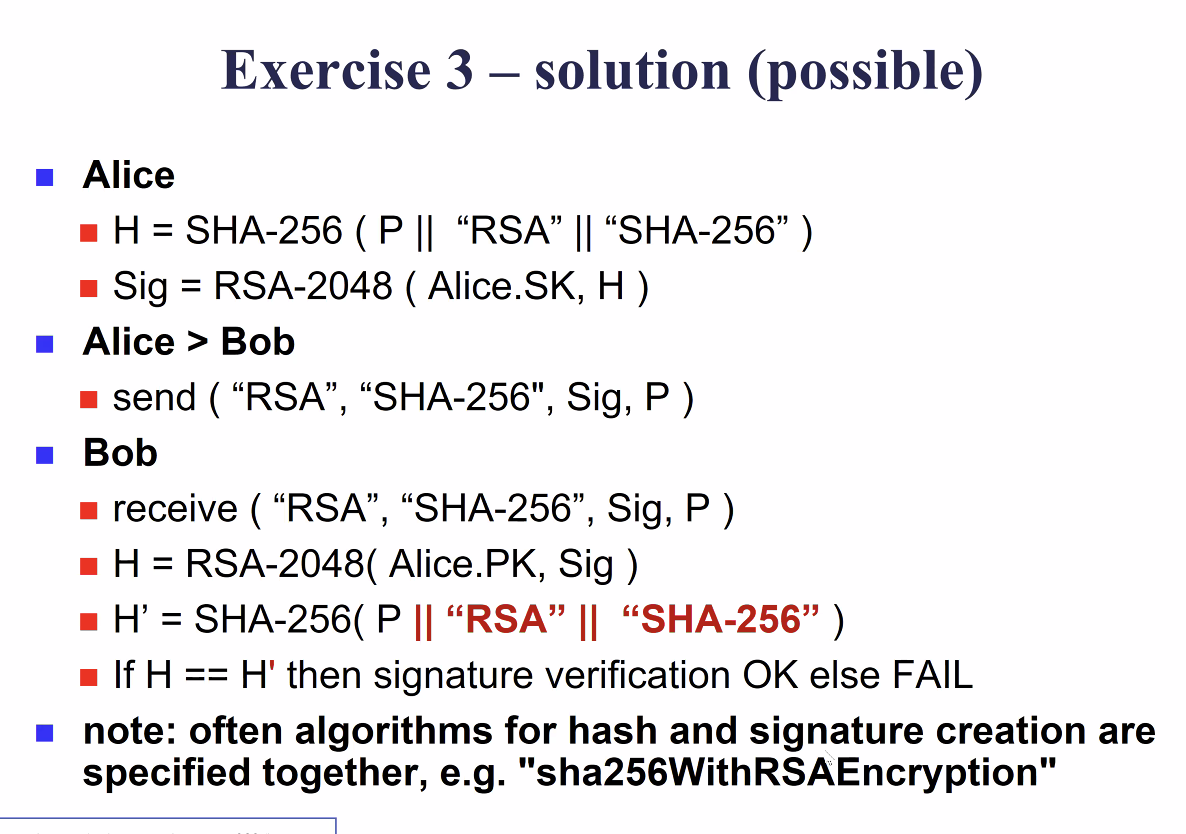
\includegraphics[width=0.5\linewidth]{res/png/ex3solut.png}
    \caption{}
    \label{}
\end{figure}


\paragraph{Another exam problem}

\begin{figure}[!ht]
    \centering
    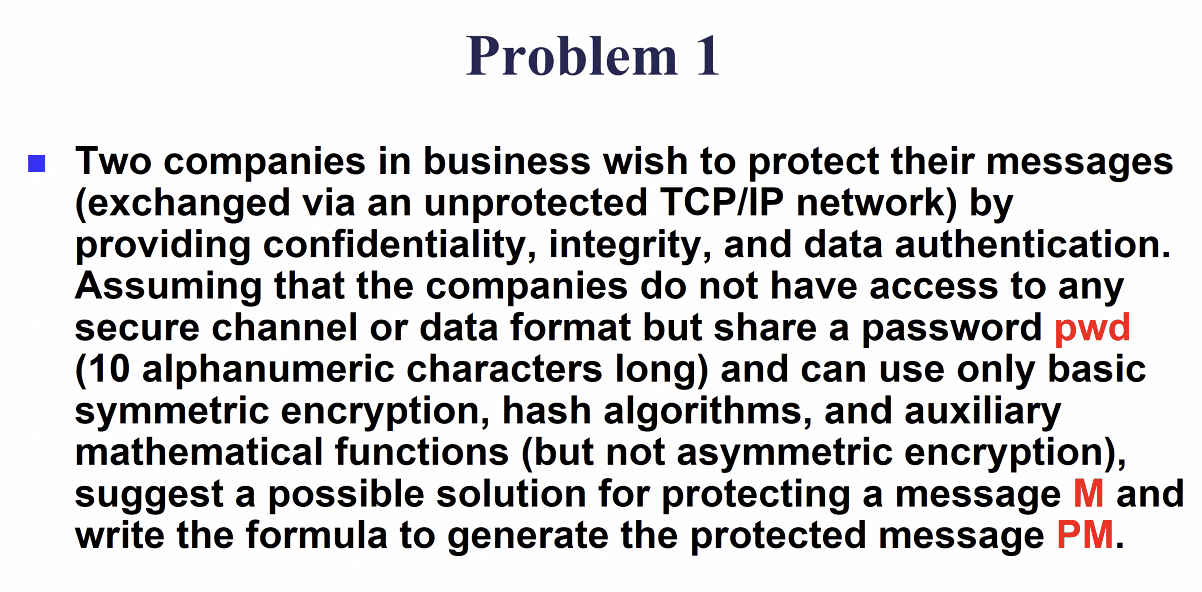
\includegraphics[width=0.5\linewidth]{res/png/exprocompanies.png}
    \caption{}
    \label{}
\end{figure}

We want to protect a message M for confidentiality, integrity and data authentication, but without asymmetric cryptography.

We have a password, but in order to protect data we need keys. We could use PBKDF to derive a key from the password.

Then, to protect data for integrity and data authentication, we can use HMAC (like sha-256).

We can use symmetric encryption (like aes-128-cbc) for confidentiality.

We must choose one between EtA, AtE, or A\&E. If for example, we choose EtA, we need to generate 2 different keys, because it's not secure to use the same for encryption and for MAC.

Now that we have all the plan, we must write all the formulas at the exam:

\begin{figure}[!ht]
    \centering
    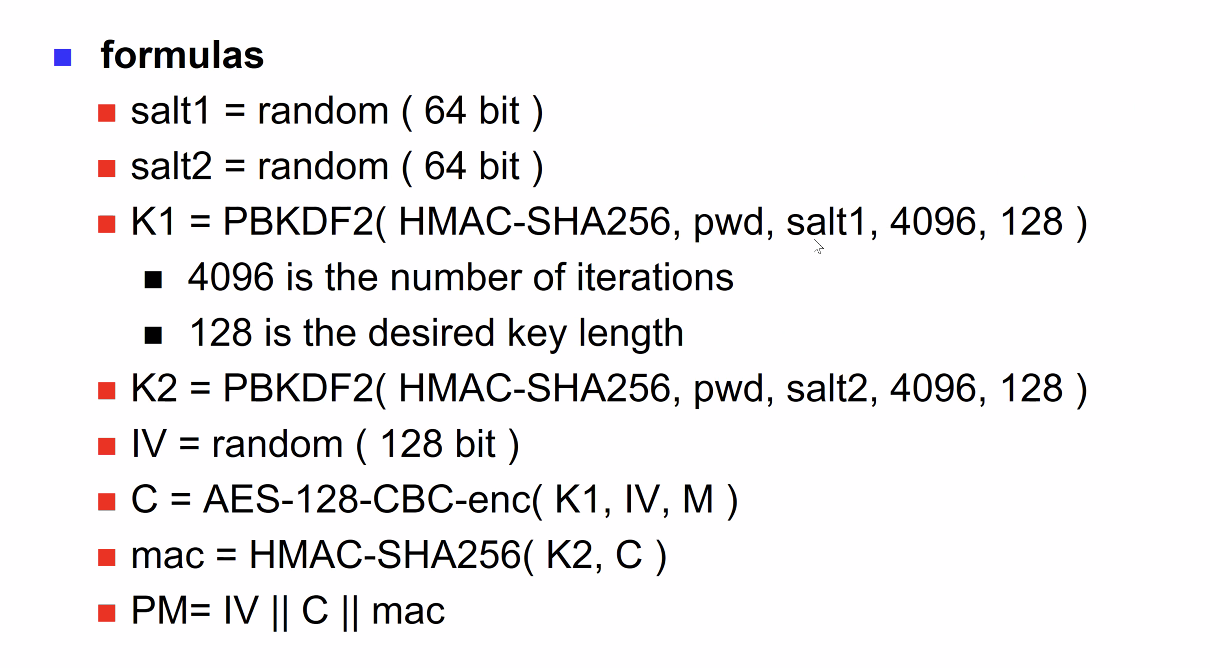
\includegraphics[width=0.5\linewidth]{res/png/formulaspart1.png}
    \caption{}
    \label{}
\end{figure}


\section{Authentication and Certificates}
\paragraph{Q1}
What is a certification authority?\\
Answer: an organization that issues public-key certificates to entities. It doesn't certify encryption algorithms or keys, nor does it distribute private keys.

\paragraph{Q2}
Assume a CA issues a X.509v3 certificate to Alice. Which of the following values are included in the certificate?

Answer:
\begin{itemize}
    \item Alice's public key (NOT the private!)
    \item A digital signature on Alice's X.509v3 certificate, calculated with the private key of the CA (NOT the public key). If the certificate wasn't signed, it would lack integrity and authentication.
    \item An indication of the owner of the certificate, such as Alice's name or e-mail address.
    \item A time period indicating the lifetime of the certificate.
    \item An indication of the issuer of the certificate, such as the CA's name.
\end{itemize}

\paragraph{Question 3}
Why would a CA revoke a certificate for a user?\\
Answer: if the subject's private key has been compromised. Also, if the user performed cyber attacks.

\paragraph{question 4}
Which of the following statements about CRL and OCSP are correct?

Answer:
\begin{itemize}
    \item CRL is a list of revoked certificates issued by a CA: the CA signs the CRL, providing it.

    \item OCSP is a protocol to query a server about the validity of a  single specific certificate at the \textbf{current time}. It has been invented to check the current validity of a certificate, for example when we do transactions! If we want to check old validity, we should use CRL.
\end{itemize}

\paragraph{Question 5}
Let's assume Alice sends a digitally signed message to Bob and attaches her X.509v3 certificate and the whole chain.

Why would she attack the certificate if she already digitally signed the message? To indicate to Bob which public key to use to verify the digital signature.

But then, which steps must Bob perform to verify the signature on the message?

Answer:
\begin{itemize}
    \item Verify the signature on the message by using the certificate of Alice
    \item verify that the certificate of Alice is authentic by constructing the chain up to a trusted CA and verifying the signatures on each certificate in the chain.

    \item verify that each certificate in the chain has not been revoked.

    \item Do not check the trusted root CA certificate that Alice sent him because he should have it already configured it as trusted. In fact, Bob can't accept a root CA that someone just sends him; he should have the root CA already configured. Because a clever attacker could otherwise send bob a fake root CA.
\end{itemize}


\end{document}
